\documentclass[12pt, letterpaper]{article}
\usepackage{graphicx}
\usepackage{geometry}
\geometry{
  a4paper,
  total={170mm,257mm},
  left=20mm,
  top=20mm,
}
\usepackage{crimson}
\usepackage[T1]{fontenc}
\usepackage[round]{natbib}
\usepackage{multirow}
\usepackage{array}
\usepackage{xltabular}
\usepackage{xcolor}
\usepackage{hyperref}
\usepackage{xurl}
\usepackage{ragged2e}

% Colour external URLs blue so they read as links; leave cross-references and
% citations black so the body text is unaffected.
\definecolor{linkblue}{HTML}{1A56B0}
\hypersetup{
  colorlinks=true,
  urlcolor=linkblue,
  linkcolor=black,
  citecolor=black,
}

% Weighted X column: L{f} takes f/(sum of f) of the available width.
% The factors must sum to the number of columns.
% \RaggedRight (ragged2e) rather than \raggedright so narrow columns can hyphenate.
\newcolumntype{L}[1]{>{\hsize=#1\hsize\RaggedRight\arraybackslash}X}

  % longtable captions default to 4in; match the table width instead.
\setlength{\LTcapwidth}{\textwidth}

% Link a ringbp GitHub issue/pull request by number, e.g. \ghissue{102} -> #102.
\newcommand{\ghissue}[1]{\href{https://github.com/epiforecasts/ringbp/issues/#1}{\##1}}
\newcommand{\ghpr}[1]{\href{https://github.com/epiforecasts/ringbp/pull/#1}{\##1}}
\newcommand{\ghcommit}[1]{\href{https://github.com/epiforecasts/ringbp/commit/#1}{#1}}

\title{Reflections on epidemiological model development in COVID-19 and since: a case study on test-trace-isolate}

\begin{document}

\maketitle

\section*{Introduction}

Responding to an emerging infectious disease threat entails trying to understand the epidemic dynamics, and increasingly that happens via formal mathematical and computational approaches. The better that understanding, the better policy- and decision-makers can take the appropriate public-health actions. The formal modelling tasks early in a disease outbreak blend predictable questions that apply in many epidemics and more idiosyncratic ones. For example, public health response organisations will predictably want to estimate the effective reproduction number ($R_t$) from incidence time series \citep{Cori2013}. While new technologies or epidemic traits like COVID-19 S-gene target failure (indicating novel variant emergence) \citep{Davies2021, Clark2022}; digital contact tracing \citep{Wymant2021}; or changes in re-infection rates \citep{Pulliam2022} raise idiosyncratic questions. \\

When an outbreak hits, the software tools needed to answer the relevant questions may or may not be available. Perhaps because they have not been developed, or because there is not a publicly available or discoverable implementation. Unfortunately, public health research has historically not incentivised robust software engineering \citep{Kucharski2020}. In the COVID-19 pandemic, the epidemiological modelling software required for predictable tasks was often unavailable, or difficult to use, and necessitated the rapid development of modelling tools \citep{BrooksPollock2021, Jombart2021, Lais2024}. In these outbreak scenarios lacking the requisite models, people hastily write code addressing the outstanding questions because working in the exponential growth phase of an epidemic, timeliness of results impacts their ability to inform response \citep{Whitty2015}. Under that time pressure, there is usually a compromise between urgency, quality, and cost. In crisis response, any scientific software engineering best practices are further degraded. The COVID-19 pandemic proved a prime example of this\footnote{We do not cite examples of poor software practices here as it is not fair on the many people who worked tirelessly to assist the COVID-19 response in a stressful environment, and poor software development was widespread as a result.}. \\

In the aftermath of the COVID-19 pandemic there has been a renewed acknowledgement by public health professionals and funders that robust modelling tools are required for preparedness and response \citep{Becker2021, DHSC2025}. In the last few years several initiatives have made improving outbreak analytics and modelling software a principal target \citep{Morgan2022, TamayoCuartero2025, CDC2026}. These initiatives have coincided with an increasing number of research software engineers (RSEs) who can develop tools in line with best practices \citep{Goth2025, Kijewska2026}. \\

In this viewpoint we reflect on the development of one particular highly influential COVID-19 epidemic model as a case study \citep{Hellewell2020}. The model and software implementation, \texttt{ringbp}, were developed in the early phase of the COVID-19 pandemic to evaluate the effectiveness of isolation and contact tracing to control seeded outbreaks \citep{Hellewell2026}. The model and the software have received post-pandemic development, undertaken mostly by authors of this paper, several of whom also authored \citet{Hellewell2020}. Herewithin we evaluate and benchmark how the model has evolved, and whether this alters the conclusions from the early COVID-19 study; reflecting on how post-pandemic, peacetime development can improve model correctness, flexibility and usability of a digital public good \citep{DPGA2025}.

\section*{Case study: intra-pandemic and post-pandemic model development}

At the start of the COVID-19 pandemic an important outstanding question was whether the outbreak could be controlled with isolation and contact tracing alone. If not, other non-pharmaceutical interventions (NPIs), such as national lockdowns, or pharmaceutical interventions, such as vaccines, would be needed to bring the $R_t$ below one for a sustained period. \\

One example of an epidemiological model developed in the first months of the COVID-19 pandemic was a contact tracing and isolation model developed to assess if such an individual-level NPI would be effective (Figure \ref{fig:timeline}) \citep{Hellewell2020}. The core transmission model is a branching process. In branching processes, an individual's infection natural history, interaction with interventions, and offspring created are drawn as samples; an infector's state may influence outcomes for their offspring, but not vice versa, and offspring are independent of each other. Well before the pandemic, branching processes were well-established mathematically \citep{Harris1963, Bailey1975}, as were their applications in epidemiology, particularly for modelling early outbreak dynamics in largely susceptible populations \citep{Diekmann2000}. Despite branching process models being established -- with existing software implementations of simulation and inference, e.g. \texttt{bpmodels} \citep{Funk2023} -- and evaluating whether contact tracing could effectively contain an epidemic being a predictable task, no consensus software implementation contained the individual-level interventions of interest early in the pandemic. Thus a COVID-19 branching process model with NPIs was written in the R package \texttt{ringbp} \citep{Hellewell2026} for the \texttt{R} language \citep{R2026}. \\

Development of the epidemiological model started in early January 2020 (Figure \ref{fig:timeline}). As the outbreak situation became clearly urgent, development switched to collaborative work on GitHub with the first commit recorded on 24th January. For context, there were only 849 confirmed COVID-19 cases in the world by this date \citep{WHO2026}. The model was inspired by code that had been written for ring vaccination in the 2014--2016 Ebola response \citep{Kucharski2016}. \\

\begin{figure}[h]
    \centering
    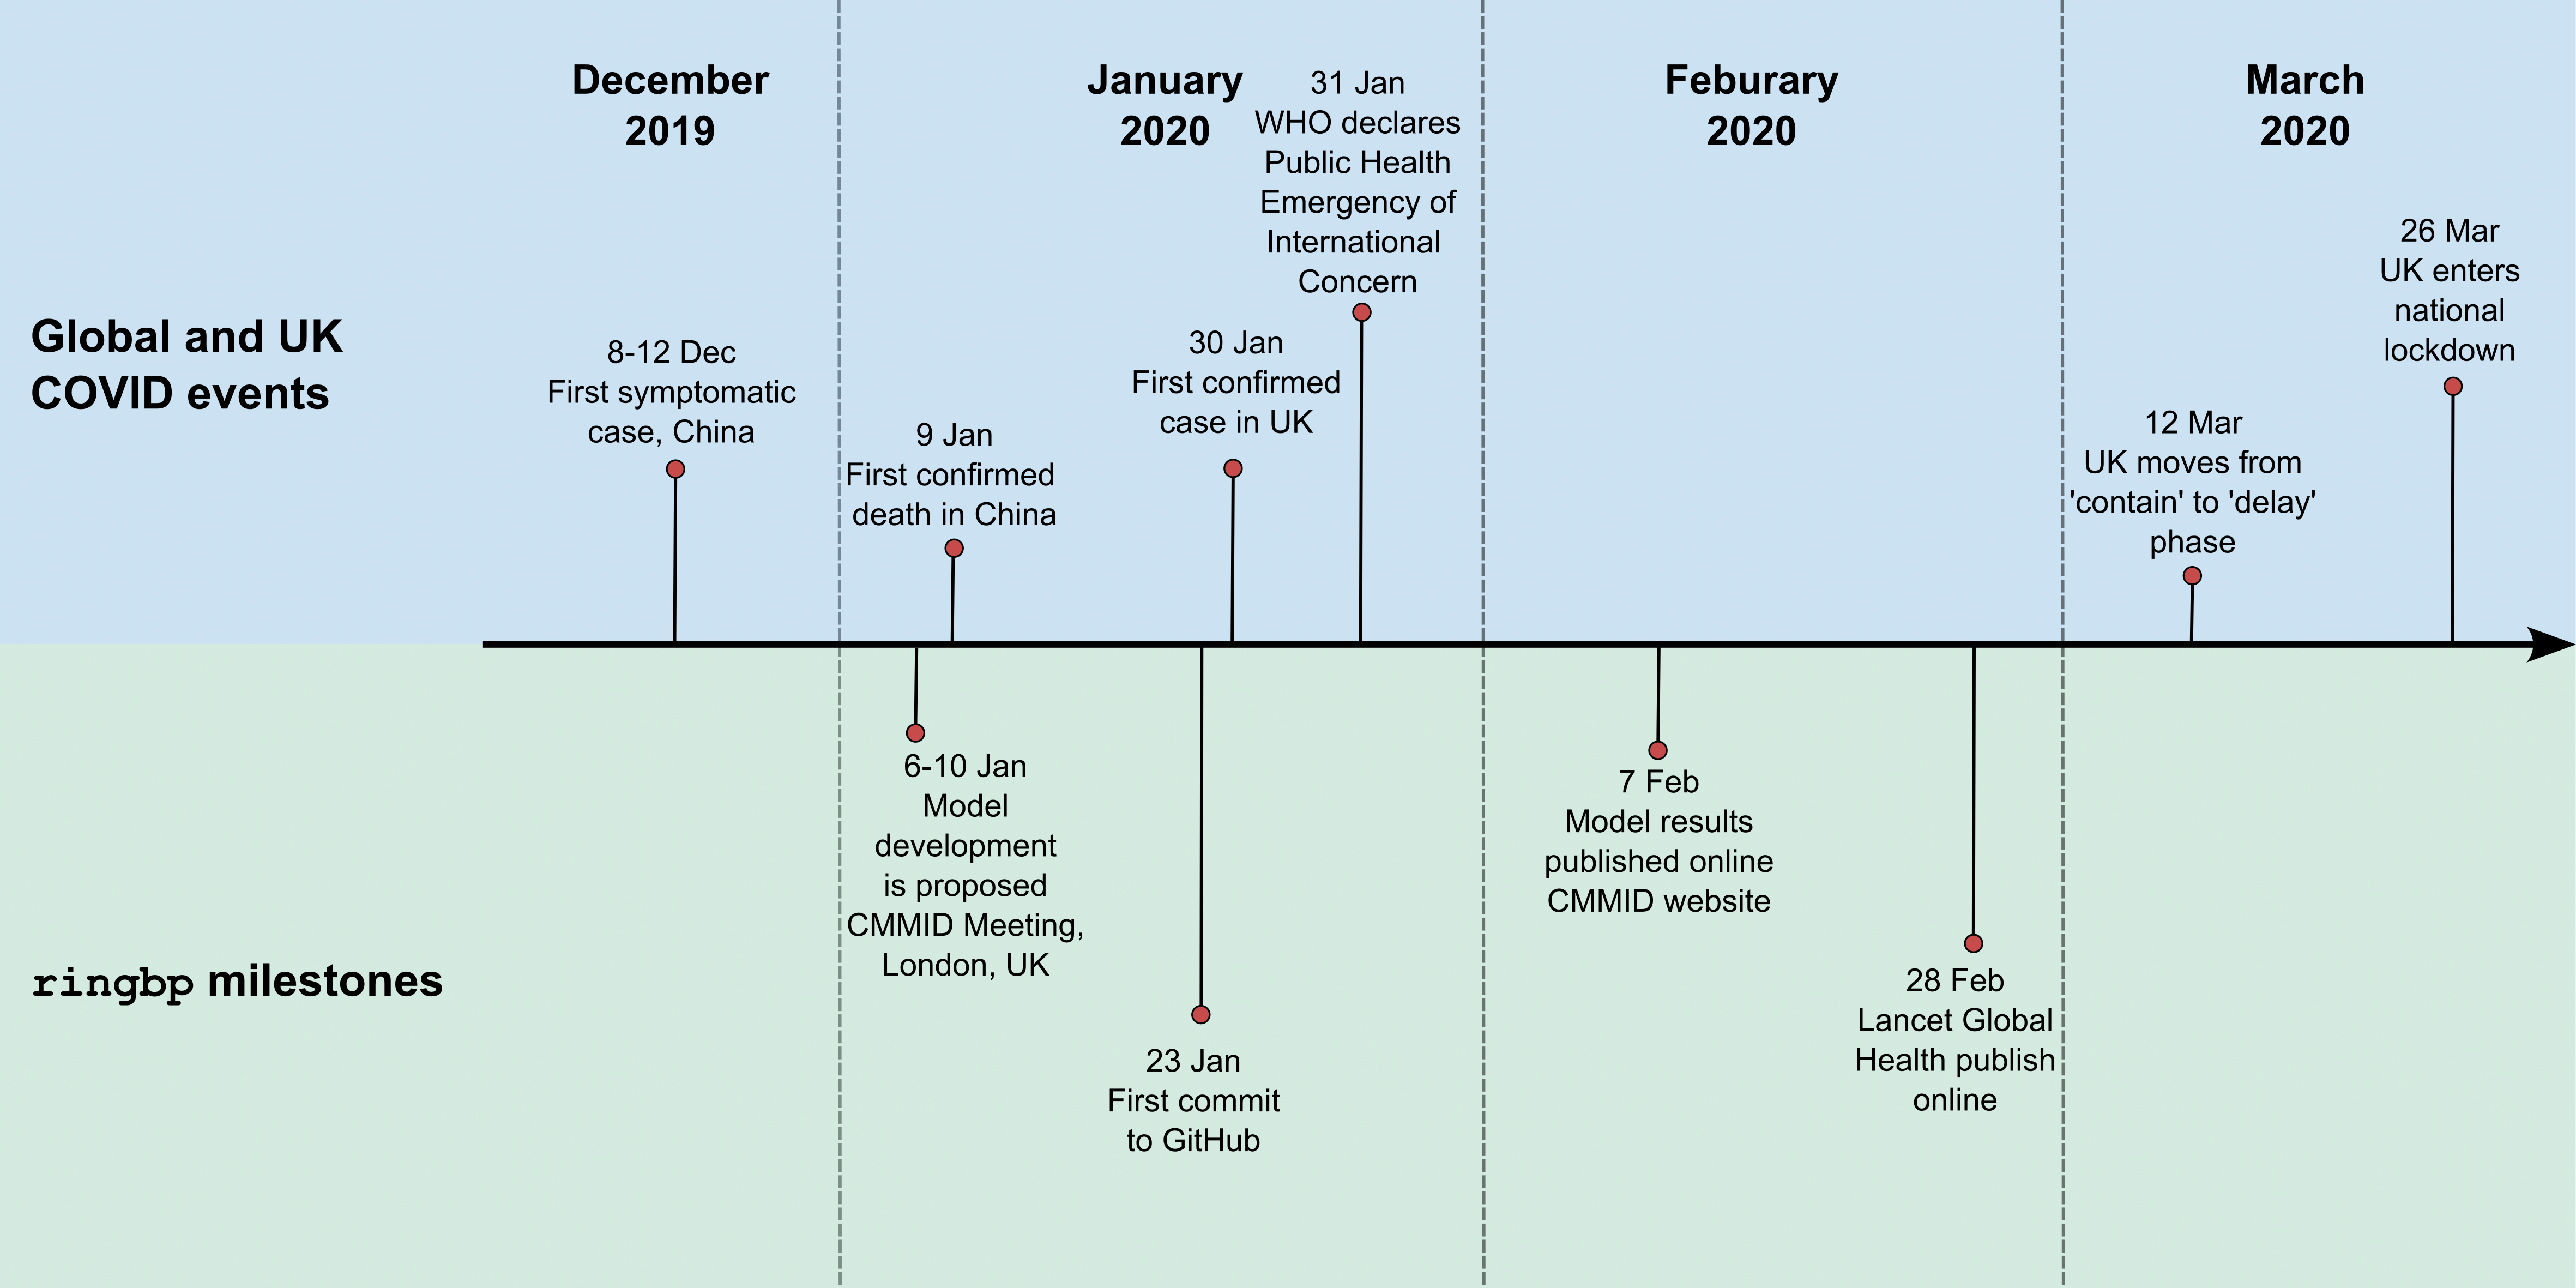
\includegraphics[width=\textwidth]{../plots/timeline.png}
    \caption{A timeline, December 2019 -- March 2020, of Global and UK events in the first months of the COVID-19 pandemic (top) and the events in the development of the ringbp COVID-19 model and publication of results (bottom). The first results were published on the CMMID website: https://cmmid.github.io/topics/covid19/contact-tracing.html. After stopping community testing in the UK on 12 March 2020, testing and contact tracing did not restart until September 2020.}
    \label{fig:timeline}
\end{figure}

The team at the London School of Hygiene and Tropical Medicine developing the epidemic model within the \texttt{ringbp} R package was led by early career researchers with support from senior epidemiologists and input from the Centre for the Mathematical Modelling of Infectious Diseases (CMMID) COVID-19 Working Group. Many of those involved were concurrently working on several aspects of pandemic response. There was no dedicated software engineering capacity during development: many team members were fixed-term researchers displaced from non-COVID epidemiological research which was not generally focused on tool development. After expedited development, \texttt{ringbp} was used to assess the effectiveness of isolation and contact tracing under various pathogen characteristics and response scenarios, and results published in \cite{Hellewell2020}. \\

\cite{Hellewell2020} informed the COVID-19 response, first as evidence in the UK pandemic response groups Scientific Advisory Group for Emergencies (SAGE) and Scientific Pandemic Influenza Group on Modelling (SPI-M) \citep{Kucharski2020a}, and later in publication with over 1,000 citations and substantial media mentions to date.\footnote{1,158 citations in the Web of Science Core Collection, 3,175 citations according to Google Scholar, and an Altmetric Attention Score of 2203, as of August 2026 (\url{https://www.altmetric.com/details/76820821}).} \\

Epidemic models can be framed as having two dimensions of correctness: 1) \textit{assumption correctness} (relevant model structure and parametrisation), and 2) \textit{implementation correctness} (bug-free model translation). Assumption correctness is the sensible construction of an infectious disease model (but applies to modeling in general), and that assumptions correctly approximate the empirical infection and transmission dynamics. Several groups wrote responses to \cite{Hellewell2020} \citep{Gurdasani2020, Mitj2020, Xiong2020}. While \cite{Eggo2020} and \cite{Hellewell2020b} clarified the limitations of the epidemic model, the responses raised important points around assumption correctness, particularly in the choice of simulation parameters and how these only represented a subset of all contact tracing and testing response strategies. Later during the pandemic, other researchers also extended the core epidemic model to include transmission through a social network \citep{Firth2020}, and behavioural response to isolation measures \citep{Davis2021}. \\

Since the pandemic the utility of the \texttt{ringbp} model and the possibility of generalising it into a framework for evaluating targeted interventions for outbreak control were recognised. The post-pandemic development that followed affected both assumption and implementation correctness, and may cause substantial differences in model output. Supplementary table \ref{tab:dev-table} outlines each of the important model developments and links to the open-source development record. In this piece we reproduce the analysis of \cite{Hellewell2020} using both the pandemic version of \texttt{ringbp} (v0.1.0) and the current version (v2.0.0) to evaluate whether the results that informed public health decision making would differ today. We quantify differences in outbreak control, measured using the probability of extinction and simulated effective reproduction number. Additionally, we compare model output directly before and after each development; this includes changes that cannot influence the results of \citet{Hellewell2020}, because they fall output the parameter space of that study. Outbreak control is measured using the probability of extinction (P(extinct)) and the simulated effective reproduction number. We also compare the computational performance of
the two versions. See the supplementary material for a full description of the
methodology. \\

\bibliographystyle{plainnat}
\bibliography{ringbpCOVID.bib}

\section*{Supplementary Material}

\footnotesize
\begin{xltabular}{\textwidth}{|L{0.3}|L{1.7}|L{1.7}|L{0.8}|L{0.75}|L{0.75}|}
\caption{The bugs and bug fixes in the ringbp R package since development restarted in the first quarter of 2025 until now (first quarter of 2026). Each row contains a brief description of the bug and the patch that attempts to resolve the bug. Development of ringbp takes place on GitHub with the use of GitHub issues as a bug tracker, and GitHub pull requests to integrate proposed changes into the codebase. The issue and pull request number(s) are also provided and linked for each row to see the history of development. This table does not include developments on package infrastructure. We categorise the change type based on the ISO/IEC 25010 Software Quality Model standard and additionally place the label based on Conventional Commits v1.0.0 specification in parentheses.}
\label{tab:dev-table} \\
\hline
Label & Problem description & Change description & Change type & GitHub issue(s) & GitHub Pull request(s) \\
\hline\hline
\endfirsthead
\hline
Label & Problem description & Change description & Change type & GitHub issue(s) & GitHub Pull request \\
\hline\hline
\endhead
\hline
\multicolumn{6}{r}{\footnotesize\itshape Continued on next page} \\
\endfoot
\hline
\endlastfoot
\multicolumn{6}{|c|}{1 Intervention} \\
\hline
1a & When quarantine was active, only symptomatic cases that test positive were quarantined when contact traced. This meant that traced contacts that were asymptomatic or tests returned a false negative were not quarantined/isolated, and did not represent an exposure-based intervention aimed at isolating infections that symptom screening and testing misses, and reducing pre-symptomatic transmission. & The model logic for quarantine is updated so when active a contact that is traced as being exposed to an infector they are quarantined/isolated at the earliest of their infectors isolation time (independent of their symptom status or a test result) and the delay from symptom onset-to-isolation. & Bug\slash Model Choice & \ghissue{227} & \ghpr{213} \\
\hline
1b & If quarantine was active, traced infectees were isolated at their infectors isolation time, even if this event time was after the time an individual became symptomatic and went into isolation after their onset-to-isolation delay. & When qurantine is active, infectees are isolated at the earliest of their infector's isolation time or the onset-to-isolation delay after becoming symptomatic. In theory, the latter could be earlier due to variability in sampling isolation delays. (N.B. quarantine was not used in \cite{Hellewell2020}). & Bug\slash Model choice & \ghissue{102} & \ghpr{107} \\
 \hline
 1c & The model assumed that all cases follow the same pathway from being infected, becoming symptomatic, and then going into isolation either after an onset-to-isolation delay or being contact traced. There was no option of a second pathway to isolation with distinct parameters. For example, it was not possible to model a response in which some individuals get tested are becoming symptomatic and isolate upon a positive test result, while other individuals do not bother testing after becoming symptomatic and instead self-isolate a delay after becoming symptomatic. This can be especially relevant in early outbreak scenarios where testing capacity is limited and stay-at-home if symptomatic guidance is issued. & New parameters were added to the model that users can specify to control the probability that an individual will self-isolate (as opposed to going to get a test), and the delay distribution between becoming symptomatic and self-isolating. The default probability of self-isolation is zero for backwards compatibility. & Enhancement & \ghissue{212} & \ghpr{213} \\
 \hline
 1d & The model fixed the targeted interventions start on day zero of the outbreak (i.e. at the same time as the infection of the index case). This prevented modeling scenarios where contact tracing or testing only starts $n$ days after the start of the outbreak. & The probability of successfully contact tracing an infectee and the test sensitivity parameters have both been updated from strictly numeric scalar inputs to functions that can be defined as any time-varying functions whose output must be $[0,1]$. This allows contact tracing and testing to activate on a user-defined day and change in any user-define function, for example increasing capacity to trace or improved test sensitivity... The model accepts numeric scalar inputs for simplicity and backwards compatibility and these are converted internally to time-constant functions. & Enhancement & \ghissue{229} & \ghpr{230} \\
 \hline
 \multicolumn{6}{|c|}{2 Epidemic model} \\
 \hline
 2a & The onset-to-isolation delay for each case in a generation is sampled from the onset-to-isolation delay distribution once and recycled for every case in that generation. This reduces the variance of the onset-to-isolation times. & The onset-to-isolation delay distribution is sampled for every individual in a generation, each getting an independent random draw from the distribution. & Bug\slash Model choice & \ghissue{94} & \ghpr{98} \\
 \hline
 2b & The latent period was hardcoded to one day. This is sensible to prevent negative generation times and given the uncertainty time between infection and infectiousness in the early phase of the COVID-19 pandemic. However, it prevents users from changing the latent period and also creates a negative? bias in the proportion of symptomatic transmission due to truncating the distribution of transmission time. & The latent period is now a user-defined parameter in the model, with a default of zero, chosen to remove any bias in the proportion of presymptomatic transmission. If the user specifies a latent period greater than zero a warning message to returned stating the realised proportion of presymptomatic transmission may be less than specified and the simulation states how the realised presymptomatic transmission differs from the user-specified value. & Model choice & \ghissue{124} & \ghpr{142} \\
 \hline
 2c & [CHECK THIS AGAINST PANDEMIC CODE] The generation time calculated from the symptom onset time (sampled from the incubation period) and the proportion of presymptomatic transmission using the skew normal distribution, was being passed the incubation period in absolute time. This had two consequences, first the latent period was in relative time, its hardcoded value of 1 day had little to no effect; second, the exposure time of some infections is before the exposure time of their infectors. & The exposure time is used when calculating the generation time to ensure the delay between exposure of an infector and infectee is non-negative. This ensures the calculation uses relative time rather than absolute time in the simulation and the minimum generation time is correctly enforced by the latent period. & Bug & \ghissue{124} & \ghpr{142} \\
 \hline
 2d & Outbreak extinction was defined as zero cases between a week range window. This has several downsides. First it falsely detects extinction is there are cases before and after the extinction window but zero cases within the window. Second it, somewhat counterintuitively, defines an outbreak as not extinct if extinction happens within the week range window. This definition was intended for \cite{Hellewell2020}. Lastly, it requires the user to modify the extinction window in accordance with the simulation duration in case the window falls outside the simulation timespan. & Extinction, as defined within the outbreak model by all infectious cases have had the opportunity to transmit but no new cases are generated, is now output with the simulated outbreak. This true extinction variable is used by default when the user does not specify a time, or timespan, for extinction. The user can optionally specify a timepoint to test whether extinction occurred by this time, and the original extinction window remains an option. & Model choice & \ghissue{132} & \ghpr{161} \\
 \hline
 2e & When cases are isolated and the basic reproduction number in isolation ($R_0^{iso}$) is greater than zero, the offspring distribution of isolated individuals is sampled over multiple generation (\texttt{generation leak}). In branching process models, each generation should be an self-contained step with all transmission and intervention events happening within the generation. This causes a differences between the user-specifying offspring distribution and the realised offspring distribution in the simulation, which becomes the sum of multiple offspring random samples over more than one generation. (N.B. \cite{Hellewell2020} fixed $R_0^{iso} = 0$). & A new offpsring sampling algorithm was implemented that samples from both the community and isolated cases offspring distributions, then all new infectees get assigned a generation time, then the community cases that have an exposure time $>$ isolation time are discarded and the isolated cases that have an exposure time $\leq$ isolation time are discarded. This encapsulates all the transmission in a single generation and multiple offspring draws is removed. & Bug & \ghissue{148} & \ghpr{169} \\
 \hline
 2f & The simulation has two stopping criteria, maximum days and maximum number of cumulative cases. These are to prevent the branching process model simulating unbounded outbreaks. The maximum number of days was tested against the latest symptom onset date in the outbreak. This meant that long incubation periods can stop the simulation, as well as stopping the simulation before later generations whose symptom onset falls before the maximum day, preventing them from transmitting and biasing outbreak size downwards. & The maximum number of days is now tested against the earliest exposure time, ensuring all new infection times are later than this. The outbreak simulation is stopped once all new infections occur after the maximum number of days from the start of the outbreak, counted from the exposure of the initial cases on day 0. & Model choice & \ghissue{163}, \ghissue{225} & \ghpr{228} \\
 \hline
 2g & The model assumed that test sensitivity was perfect. This is a reasonable assumption went modelling polymerase chain reaction (PCR) testing in an outbreak for infected individuals to isolate, as was done in \cite{Hellewell2020}. However, it restricts modelling different testing strategies that may also be application in outbreak response, such as lateral flow tests (LFTs), as mentioned by \cite{Gurdasani2020}. Varying test sensitivity was added as part of the \cite{Davis2021} work in extending a fork of \texttt{ringbp}, but this feature was never merged into the \texttt{ringbp} model. & A test sensitivity parameter specifying the probability of a test result being a true positive has been added to the model to enable some tests to return false negative results and these infected individuals are not isolated and their contacts are not traced. The test sensivity parameter defaults to one so is backwards compatible with the perfect sensitivity scenario. & Enhancement & \ghissue{176}, \ghissue{231} & \ghpr{196}, \ghpr{232} \\
 \hline
 \multicolumn{6}{|c|}{(3) User interface and flexibility} \\
 \hline
 3a & Update hardcoded COVID-19 parameters to flexibility user-interfacing parameters & The incubation period was hardcoded to be Weibull distributed with paramters shape ($k = 2.322737$) and scale ($\lambda = 6.492272$) and the onset-to-isolation delay distribution was hardcoded to be Weibull distributed, but in this case the parameters could be specified by the user. & Enhancement & \ghissue{59} & \ghpr{84} \\
 \hline
 3b & Epidemiological and simulation control parameters were all in flat, complex function signature. Limiting model extensions and usability by ever expanding list of model arguments. & The outbreak simulation arguments have been grouped into categories and each category has a helper function (\texttt{*\_opts()} for a modular user-interface. & Enhancement & \ghissue{65} & \ghpr{127} \\
 \hline
 3c & User-defined arguments were not checked meaning that the code could error in unexpected and return uninformative errors to the user. & Input checking was added to all user-defined parameters to ensure they are epidemiologically and computationally correct. & Enhancement & \ghissue{91} & \ghpr{127} \\
 \hline
 3d & The proportion of presymptomatic transmission was defined by the user via the shape/slant ($\alpha$) parameter. This required user knowledge on how the parameter was converted into the proportion of presymptomatic transmission, and had an uninformative parameter name (\texttt{k}). & Allow the user to directly define the proportion of presymptomatic transmission and calculate $\alpha$ internally using numerical optimisation. & Enhancement & \ghissue{119} & \ghpr{123} \\
 \hline
 \multicolumn{6}{|c|}{(4) Performance} \\
 \hline
 4a & Sampling random events and condition handling was not optimised. Sampling random events was coded as \texttt{as.logical(\allowbreak rbinom(...))}, which can be improved by using \texttt{runif(x) < y}. The performance of condition handling has been improved both by the way the condition code is written and also using faster functions with equivalent functionality. & NOT SURE IF THIS CAN BE TESTED AS IT IS BUNDLDED WITH OTHER CHANGES & Enhancement & \ghissue{90}, \ghissue{92} & \ghpr{98} \\
 \hline
 4b & The data output from the outbreak scenario simulation did not efficienctly store data on outbreak generations and the effective reproduction number, with them being duplicated in the tabular (\texttt{data.table}) output for each outbreak replicate. & The outbreak scenario simulation now returns a list of two tabular data structures, an outbreak time series and outbreak statistics, to remove any duplicated data and reduce the memory footprint. & Enhancement & \ghissue{237} & \ghpr{239} \\
 \hline
 \multicolumn{6}{|c|}{(5) Testing and correctness} \\
 \hline
 5a & Testing coverage across the package was ??\% and there were minimal tests for correctness for the epidemic model code & Correctness tests were added as well as ... & ??? & \ghissue{100} & ??? \\
 \hline
 \multicolumn{6}{|c|}{(6) Documentation} \\
 \hline
 6a & Package documentation was sparse and inconsistent and lacked long-form documentation & Comprehensive, and consistently formatted function documentation has been added, long-form documentation (vignettes) have been added, ... & Enhancement & \ghissue{111}, \ghissue{139}, \ghissue{140} & \ghpr{188}, \ghpr{201} \\
 \end{xltabular}
\normalsize

\subsection*{Supplementary methods}

\subsubsection*{Examining the effect of quarantine (1a \& 1b)}

To examine the impact of the change in implementation of quarantine between pandemic and current versions of \texttt{ringbp} we run a comparison of the \cite{Hellewell2020} analysis, but with quarantine active (N.B. quarantine is inactive in all \cite{Hellewell2020} simulations). We compare the difference in the probability of outbreak extinction and the effective reproduction number from each simulation version. \\

We also isolate the differences caused by the changes in 1a and 1b individually. For 1a we run a parameter sweep over both the proportion of asymptomatic cases and probability that contacts are traced, from 0 to 1, at intervals of 0.2. This is carried out using the \texttt{ringbp} model directly before the change and directly after the change. All other model parameters are kept constant at the \cite{Hellewell2020} central values. For 1b we alter the onset-to-isolation delay mean between 2 and 12 days, at intervals of 2 days, and standard deviation between 1 and 6 days, at intervals of 1 day. Quarantine is active and it is assumed that no cases are asymptomatic and all contacts are traced. All other parameters are kept constant at the \cite{Hellewell2020} central values. We compare the differences in probability of outbreak extinction and effective reproduction number from before and after each change. \\

\subsubsection*{Examining the effect of epidemic model developments}

To test the effect of the recycled onset-to-isolation delays for each individual in an outbreak generation we conduct two analyses. The first reproduces the analysis of \cite{Hellewell2020}, using the \texttt{ringbp} directly before (\ghcommit{22f3fe99}) and directly after the fix (\ghcommit{4c47d996}). The second analysis varies the standard deviation of the onset-to-isolation distribution between 1 and 6 days, at intervals of 1 day, and runs outbreak simulations with the \texttt{ringbp} model directly before and after the change to quantify the difference in probability of extinction and reproduction number of the simulated scenarios. \\

All outbreak simulation scenarios are run for 5000 replicates to capture the variability from the stochastic simulation. \\

\subsection*{Supplementary results}

\begin{table}[h!]
\centering
  \caption{Benchmarking of changes...}
  \label{tab:benchmark-table}
 \begin{tabular}{|c|c|c|}
 \hline
 Label & $\Delta$ P(extinct) & ??? \\
 \hline\hline
 1a & 999 & Change A \\
 \hline
 1b & 999 & Change B \\
 \hline
 \end{tabular}
\end{table}

\end{document}
